\documentclass{beamer}
\usetheme{Frankfurt}
%\usecolortheme{seahorse}

\title
{Polarized Neutron Scattering}
\author
{Walter Van Herck\inst{1}}
\institute[JCNS at MLZ] % (optional)
{
  \inst{1}%
  J\"ulich Centre for Neutron Science at MLZ
}
\date[BornAgain] % (optional)
{BornAgain School and User Meeting, 2018}
\subject{Computer Science}

\begin{document}

\frame[plain]{\titlepage}

\begin{frame}
    \frametitle{Overview}
    \tableofcontents
\end{frame}

\section{Theory}

\begin{frame}
    \frametitle{Approximations}
    \begin{itemize}
        \item Elastic scattering: time-independent Schrödinger equation
        \item Far field Green's function
        \item First order in perturbation potential
        \item Small angle scattering: locally constant perturbation potentials
    \end{itemize}
\end{frame}

\begin{frame}
    \frametitle{Theory}
    \begin{itemize}
        \item First, we solve the perfectly smooth multilayer in the presence\
              of magnetization in the layers.
        \item Then we use the Green's function method to obtain the first order\
              contribution to the scattering amplitude.
        \item For magnetic dipoles, the scattering depends only on the\
              magnetization perpendicular to the wavevector transfer:
        \[ \delta v_\perp(\mathbf r) \sim \sigma \cdot \mathbf{m_\perp}(\mathbf r)\]
    \end{itemize}
\end{frame}

\begin{frame}
    \frametitle{Homogeneous solution}
    \begin{itemize}
        \item The magnetic fields will cause birefringence of the plane waves.
        \item The Green's function will again contain the homogeneous solution\
              as a function of the source location $\mathbf s$.
    \end{itemize}
    \begin{figure}
        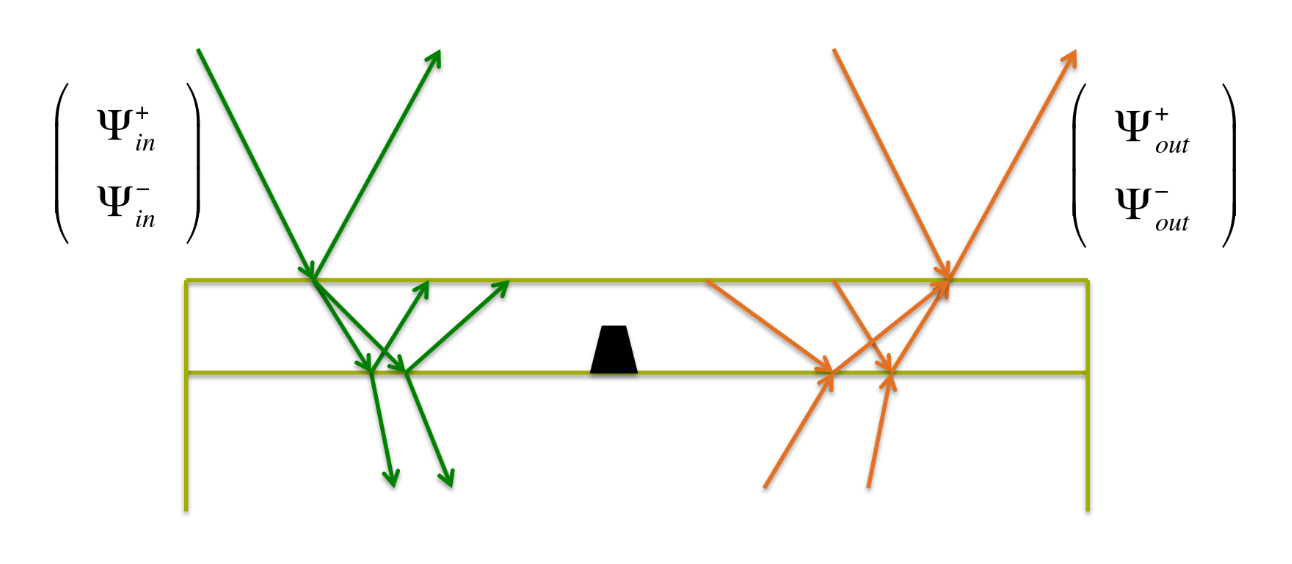
\includegraphics[width=10cm]{birefringence.png}
        \\ Birefringence of homogeneous solution
    \end{figure}
\end{frame}

\section{BornAgain}

\begin{frame}
    \frametitle{Required parameters for magnetic neutron scattering}
    \begin{itemize}
        \item Magnetic materials for layers and/or particles
        \item Beam polarization
        \item Detector polarization analysis
    \end{itemize}
\end{frame}

\begin{frame}
    \frametitle{Magnetic materials}
    \begin{itemize}
        \item Magnetic materials are defined by their magnetization in $A/m$.
        \item The external guide field is a parameter of the multilayer and\
              is also expressed in $A/m$.
        \item In both cases, one needs to input the three different components\
              of the magnetization (along the three principal axes).
    \end{itemize}
\end{frame}

\begin{frame}
    \frametitle{Beam polarization}
    \begin{itemize}
        \item A spin $1/2$ particle's state is fully determined by its density\
              matrix, which is positive semidefinite, Hermitian, trace $1$:
    \end{itemize}
    \[ \hat\rho = \sum_j p_j \left| \psi_j \rangle\langle \psi_j \right| \]
    \begin{itemize}
        \item The density matrix can be defined by its Bloch vector $\mathbf a$:
        \[ \hat\rho = \frac{1}{2}\left( I + \sigma\cdot\mathbf a \right) \]
              with $|\mathbf a| \leq 1$.
        \item The length $a=\left| \mathbf a \right|$ determines the probability\
              for the spin to be in the direction $\mathbf a$ (and thus also of\
              the opposite state):
        \[ p_+ = \frac{1}{2}\left( 1 + a \right) \]
    \end{itemize}
    
\end{frame}

\begin{frame}
    \frametitle{Polarization analysis}
    \begin{itemize}
        \item Orientation of polarization analysis: unit vector $\mathbf{\hat u}$.
        \item Transmission ratios of up and down components: $T_+$ and $T_-$.
        \item Efficiency:
              \[ P_{eff} = \frac{T_+ - T_-}{T_+ + T_-} \]
        \item Total transmission:
              \[ T_{total} = \frac{T_+ + T_-}{2} \]
    \end{itemize}
\end{frame}

\section{BornAgain GUI demo}

\begin{frame}
    \begin{center}
        \LARGE{BornAgain GUI demo}
    \end{center}
\end{frame}

\end{document}